\section{Overall description}
\label{sect:overalldescription}

Here you can see how to include an image in your document.

\begin{sidewaysfigure}
\centering
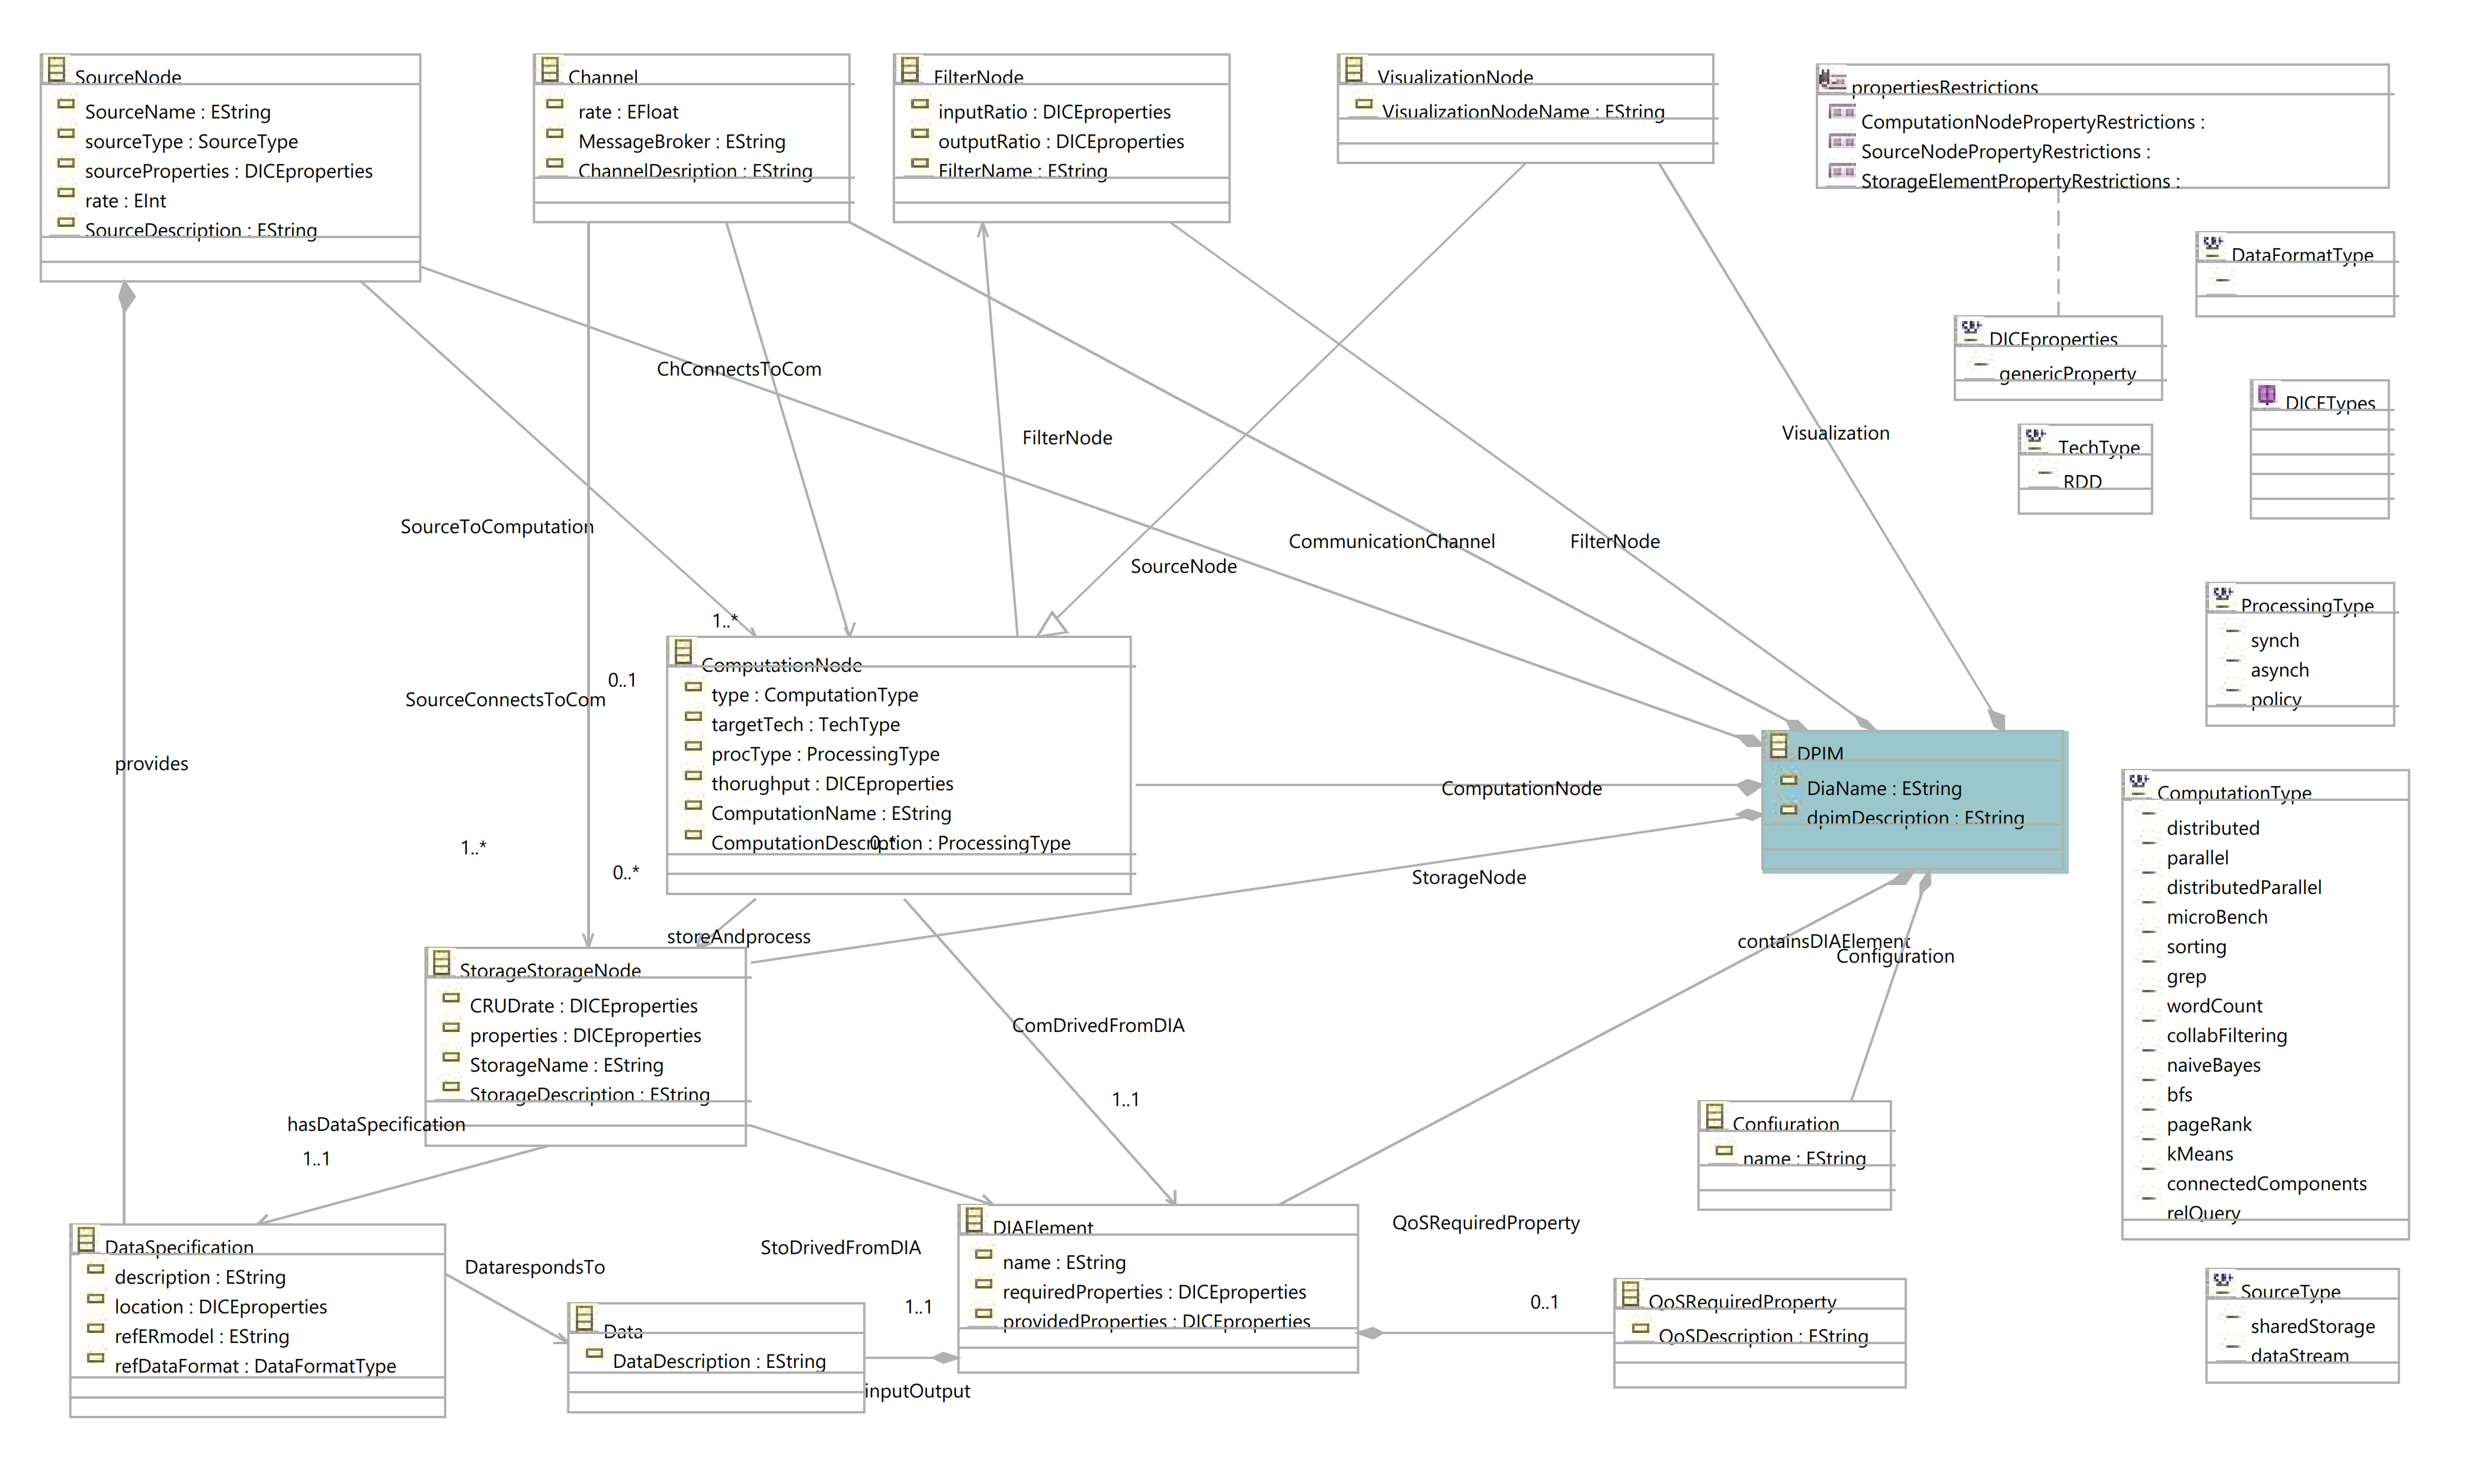
\includegraphics[width=\textwidth]{Images/11.png}
\caption{\label{fig:metamodel}DICE DPIM metamodel.}
\end{sidewaysfigure}

\begin{figure}
\centering
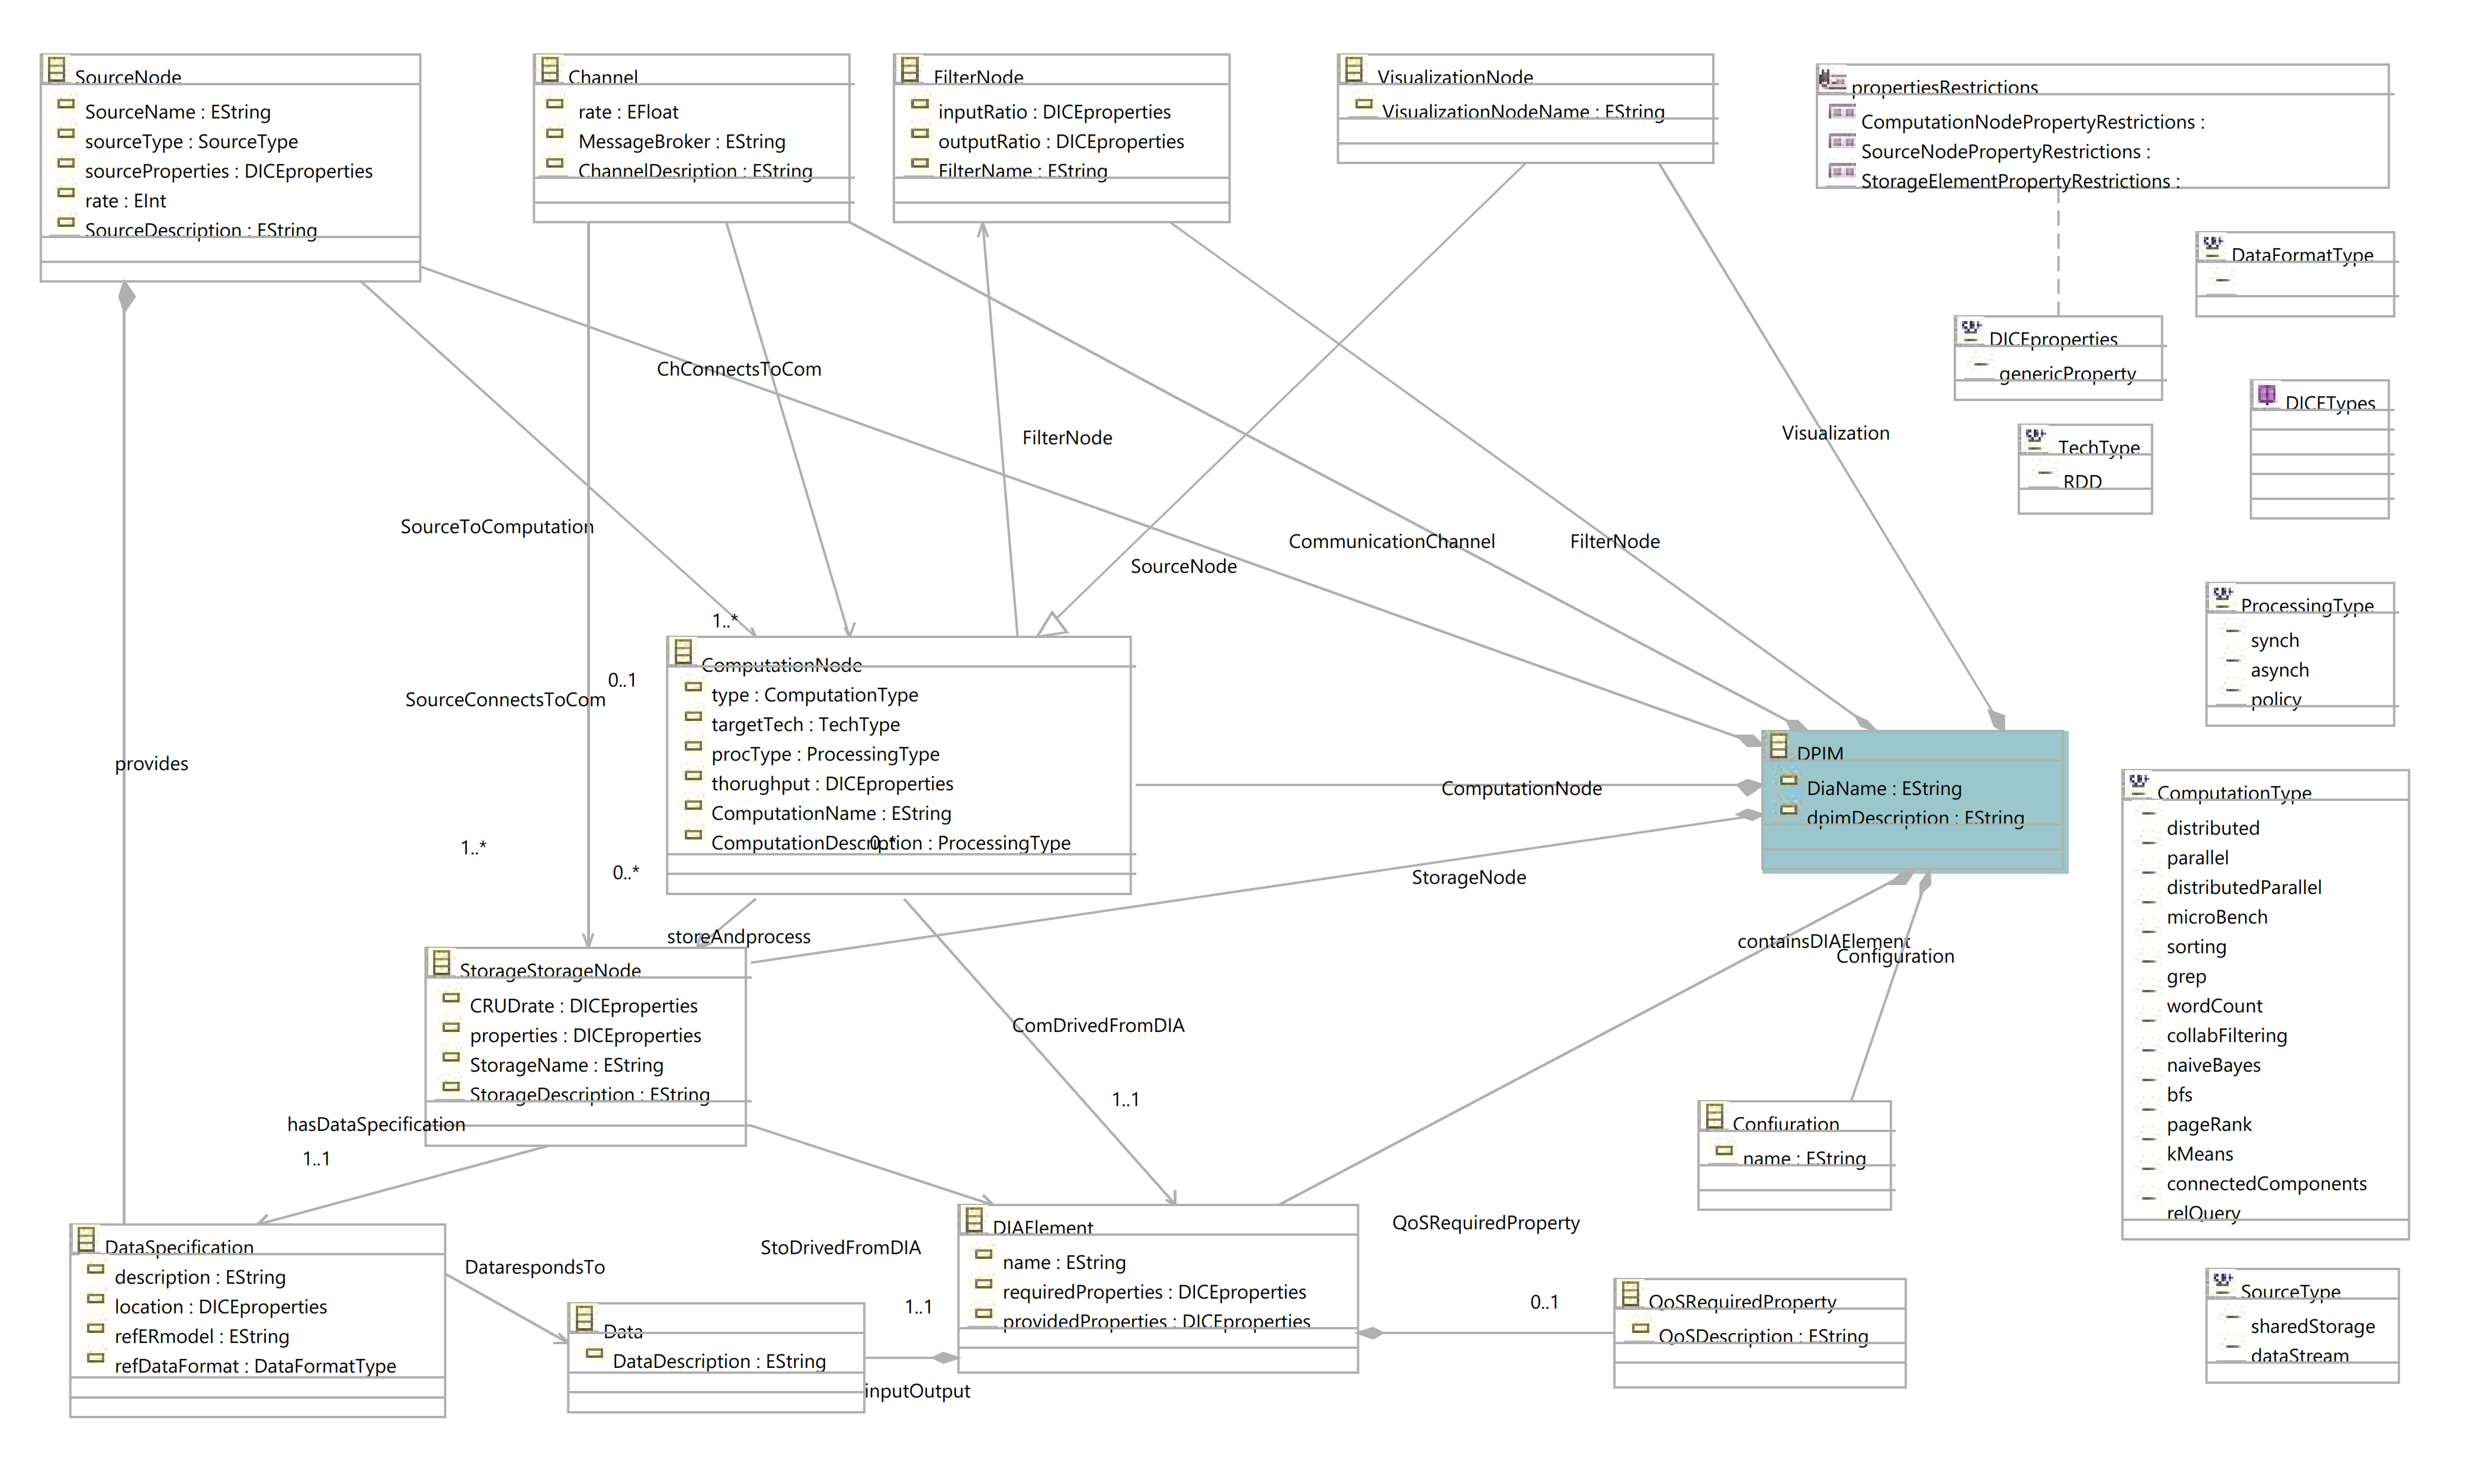
\includegraphics[width=\textwidth]{Images/11.png}
\caption{\label{fig:metamodel2}DICE DPIM metamodel in portrait form.}
\end{figure}

\subsection{Product perspective}
\label{subsect:productperspective}

Here we include scenarios and further details on the shared phenomena and a domain model (class diagrams and statecharts).

Describes external interfaces: system, user, hardware, software; also operations and site adaptation, and hardware constraints

\subsubsection{scenarios}
\label{subsubsect:scenarios}

“A narrative description of what people do and experience as they try to make use of computer systems and applications”.
A concrete, focused, informal description of a single feature of the system to be.

Heuristics for finding scenarios:
\begin{itemize}
    \item Which user groups are supported by the system to perform their work?
    \item What are the primary tasks that the system needs to perform?
    \item What data will the actor create, store, change, remove or add in the system?
    \item What external changes dows the system need to know about?
    \item What changes or events will the actor of the system need to be informed about?
\end{itemize}

\subsubsection{Use cases}
\label{subsubsect:usecases}

Here we generalize scenarios. Keep use cases small (no more than two/three pages).
Srtucture the description in terms of:
\begin{itemize}
    \item use case name: verb that indicate what the user is trying     to accomplish;
    \item participating actors;
    \item entry condition;
    \item flow of events: The steps accomplished by actors and those accomplished by the system should be clearly distinguished and the causal relationship between steps should be clear;
    \item exit condition;
    \item exceptions;
    \item special requirements (constraints, nonfunctional requirements).
\end{itemize}


\subsubsection{further details on shared phenomena}
\label{subsubsect:furtherdetailsonsharedphenomena}

\subsubsection{domain model: class diagrams and statecharts}
\label{subsubsect:domainmodel}

What should we model? The objects and people that are of interest for the given problem. The relevant phenomena. The goals, requirements, and domain assumptions.

How do we find objects? Analyze any description of the problem, the application domain, the scenarios and use cases. 

to model dynamic behavior of a single object we use state machine diagram.

From the flow of events in the use case or scenario, proceed to the sequence diagram. A sequence diagram is a graphical description of objects participating in a use case or scenario using a DAG (directed acyclic graph) notation.

Consider using state diagrams and activity diagrams.

What is the structure of the world? $\rightarrow$ Create class siagrams for static information models (UML). Is there any state change in an object that is to be defined explicitly? $\rightarrow$ Create state diagrams for dynamic class behavior models. How is the expected interaction between the software to be and the environment? Create sequence diagrams from use cases for dynamic object behavior instance examples; or create activity diagrams when you want to highlight important process.

UML does not help us in expressing assertions, we can complement its usage with some formal or informal description of these assertions.

\subsection{Product functions}
\label{subsect:productfunctions}

Here we include the most important requirements.

\subsection{User characteristics}
\label{subsect:usercharacteristics}

Here we include anything that is relevant to clarify their needs.

\subsubsection{Actors}
\label{subsubsect:actors}

Customer: a person who grocery shops.
Unregistered user: a customer using CLup without being registered. They can join the virtual queue and ask/receive updates.
Registered user/User: a customer using Clup and who is registered on the system. They can join the virtual queue, book a shopping session and ask/receive updates.
Shop manager: a person who register their shop on Clup. A shop manager can register multiple shop on the system.
Shop: a grocery shop registered on the system. It updates periodically the people present in the store and sends updates to the manager.

\subsection{Assumptions, dependencies and constraints}
\label{subsect:assumptionsdependenciescostraints}

\subsubsection{Domain Assumptions}
\label{subsubsect:domainassumptions}

Here we include domain assumptions.

Identify the relevant environment phenomena ("relevant" with respect to the goals). They are real world properties. They do not depend on the machine.

\subsubsection{Constraints}
\label{subsubsect:contraints}

Constraints: imposed by the client or the environment in which the system operates. 

Anything that will limit the developer’s options (e.g. regulations, reliability, criticality, hardware limitations, parallelism, etc.)

